\documentclass[11pt]{article}

\usepackage{amssymb,amsmath,amsfonts,amsthm,MnSymbol,graphicx,enumitem}


\theoremstyle{definition}
\newtheorem{problem}{Problem}
\usepackage{fancyhdr}
\pagestyle{fancy}
\fancyhf{}
\setlength{\headheight}{0pt}
\renewcommand{\headrulewidth}{0pt}
\rhead{Name: \underline{\hspace{1.5 in}} }
\lhead{
Math 1075\\
Instructor: Sam Kim\\
Quiz 8}

\begin{document}

\section*{}
Section 9.5, 10.1, 10.2\\
This quiz is worth 10 points and you will have 10 minutes to complete it.\\
Please show all relevant work. \textbf{Answers without supporting work will receive no credit}.\\
Good luck!
%\begin{center}
%Potentially Useful Formula
%\end{center}
%\[
%x = \frac{-b\pm \sqrt{b^2 - 4ac}}{2a}
%\]
\begin{problem}[4 points] Suppose Sam has 20 ft of fencing with which he can build a rectangualr garden. Let $x$ represent the length of the garden and let $y$ represent the width.\\ 

\noindent (a) Write an inequality representing the fact that the total perimeter of the garden is at most 20 ft.

\vspace{4em}

\noindent (b) Sketch part of the solution set for this inequality that represents all possible values for the length and width of the garden (Hint: Note that both the length and the width must be positive)

\begin{figure}[htbp]
    % Replace "my_image" with your actual file name (without extension)
    \centering
    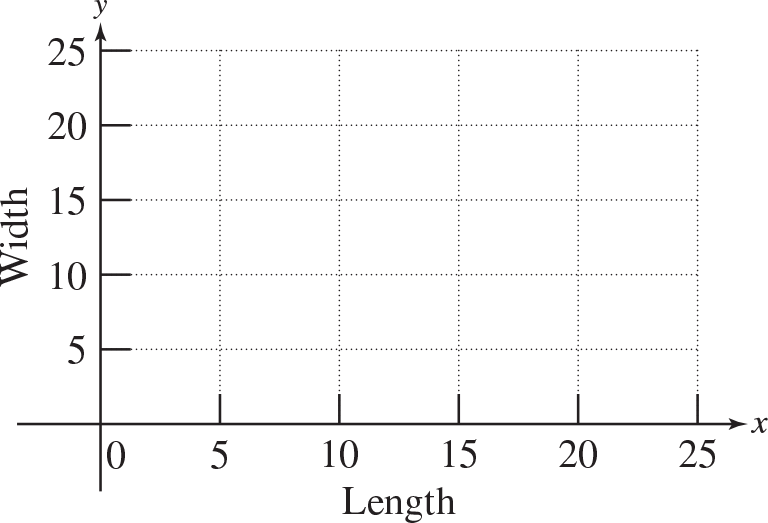
\includegraphics[width=0.6\linewidth]{mil73537_se_sec_pra_exe090561.png} 
\end{figure}

\end{problem}

\vspace{2in}

\section*{}

\begin{problem}[3 points] Simplify the expressions. Assume all variables are positive real numbers. 
\[\sqrt[4]{81x^{12}y^8}\]

\end{problem}

\vspace{2in}

\section*{}

\begin{problem}[3 points] Simplify the expressions by using the properties of rational exponents. Write the final answers using positive exponents only.
\[\left(\frac{8x^{3}y}{27xy^{-6}}\right)^{1/3} \]



\end{problem}
%%\begin{problem}[2 Points]
%%Create the graph of a continuous function $f$ such that
%%\[
%%f^{'}(x) \equiv
%%        \begin{cases}
%%        -2  & \text{if $x < -1$} \\
%%        \ \ 0 & \text{if $-1 < x < 2$}\\
%%        -1 & \text{if  $x > 2$}
%%        \end{cases}
%%\]
%%\end{problem}
%%\vspace{1.5in}
%\begin{problem}[2 Points]
%Find both $y'$ and $y''$ of $y = 5x^4 + 7x - \frac{1}{x^2}$.
%\end{problem}
%\vspace{1.5in}
%\bigskip
%\begin{problem}[3 Points]
%Find the derivative of the function $f(x) = -4x^2e^{3x}$.
%\end{problem}
\end{document}